\section*{Appendix}

\section{Ethics Statement}
This work exclusively leverages publicly available open-source datasets that have been previously established and validated in academic research. No new text, video, or audio materials are generated or incorporated as part of this study. The datasets utilized are strictly intended for research purposes and are not employed for any commercial applications.


\section{Reproducibility Statement}
To ensure the research community can replicate our findings, this project will be released as open-source software. The methodology is described in detail in Sec.\ref{method}, while Sec.\ref{exp:setting} and Appendix~\ref{ap:hyper} outline the complete training protocols and implementation details, including all hyperparameter settings.

\section{Use of Large Language Models}

During the preparation of this manuscript, we utilized large language models—GPT-5~\citep{openai2025gpt5}—exclusively to refine the language, focusing on improving grammar, flow, and tone at the sentence and paragraph levels. These tools were not employed to generate ideas, design experiments, or draw conclusions. All technical content, methodologies, and interpretations were independently written, thoroughly verified, and approved by the authors. To minimize the risk of factual inaccuracies or citation errors, every model-edited sentence underwent human review, and all references were carefully cross-checked with their primary sources. The authors accept full responsibility for ensuring the accuracy and integrity of this manuscript.

\section{Related Work}\label{related}

\paragraph{Reinforcement Learning for LLMs}

Recent efforts have focused on enhancing reasoning in LLMs using RL~\citep{slow-thinking,sft-rl-study}. DeepSeekMath~\citep{grpo} improves mathematical reasoning by continuing pre-training on math-intensive data and introducing Group Relative Policy Optimization (GRPO)~\citep{grpo}. Building on this, DeepSeek-R1~\citep{deepseek-r1} demonstrates that RL alone can drive strong reasoning, achieving performance comparable to proprietary models with large-scale training. Complementary system-level contributions, such as DAPO~\citep{dapo}, offer an open-source RL framework with a decoupled optimization strategy, achieving competitive results through a simplified training pipeline. GSPO~\citep{gspo} stabilizes RL training and reduces variance through sequence-level optimization, proving effective in large-scale mixture-of-experts models. HybridFlow~\citep{hybridflow} introduces a flexible RLHF framework with hybrid control flow and a 3D-HybridEngine. Together, these works demonstrate significant progress in advancing LLM reasoning with RL.


% Quantization of Large Language Models (AWQ, GPTQ, QAT,....)
\paragraph{Quantization for LLMs}
Quantization is a key technique for compressing LLMs, improving efficiency by reducing parameter precision. The most common approach, Post-Training Quantization (PTQ)~\citep{dettmers2022gpt3,frantar2022gptq,xiao2023smoothquant,shao2023omniquant,lin2024awq}, transforms pre-trained models cost-effectively without retraining. Recent work has pushed quantization to ultra-low bit-widths while maintaining performance~\citep{huang2024slim,dettmers2023spqr,shang2023pb,huang2024billm,liao2024apiq,tseng2024quip,huang2024mixture}, including advancements in Quantization Aware Training (QAT) to improve robustness~\citep{liu2023llm,chen2024efficientqat}. Additionally, novel precision formats like NF4~\citep{qlora}, FP4~\citep{tseng2025training,chmiel2025fp4}, and MXFP4~\citep{chmiel2025fp4} enable accurate weight representation, achieving high compression with minimal or improved accuracy loss. NVFP4~\citep{nvidia2024blackwell} is a groundbreaking 4-bit floating-point format introduced with NVIDIA's Blackwell GPU architecture. This format expands on the idea of compact, low-bit "micro" floating-point representations, offering developers enhanced versatility by adding another flexible option for their projects~\citep{zhang2025sageattention3,castro2025quartet,lee2024amxfp4}.


% Parameter Efficient FineTuning (Lora, Prefix-tuning, Q-LoRA, LongLoRA, Tina)
\paragraph{Efficient Fine-tuning}
Efficient fine-tuning is pivotal for adapting LLMs with minimal computational cost. LoRA~\citep{lora} pioneered this approach by adding low-rank adapters to frozen weight matrices. DoRA~\citep{dora} improved upon this by decomposing weight updates into directional and magnitude components, addressing low-rank constraints and enhancing stability. QLoRA~\citep{qlora} integrated LoRA with 4-bit quantization to further reduce resource usage, while LongLoRA~\citep{longlora} introduced fine-tuning methods for long-context processing. Tina~\citep{tina} demonstrated that compact models could gain reasoning ability through RL with LoRA. Beyond the LoRA family~\citep{lora}, other efficient fine-tuning techniques include prompt tuning, prefix tuning, IA3, BitFit, Fisher-masked tuning, and input-tuning~\citep{prompt-tuning,prefix-tuning,ia-3,bitfit,fisher-mask,input-tuning,guo2023lq}. These advancements underscore the importance of efficient fine-tuning for practical LLM adaptation.



\section{Experiment Hyperparameters}\label{ap:hyper}

\paragraph{Training Data and Reward Function} We trained the Qwen2.5-3B-Instruct, Qwen2.5-7B-Instruct, Qwen2.5-14B-Instruct, and Qwen2.5-32B-Instruct models, which are widely used for evaluating reasoning capabilities. Unlike other studies that rely on math-specialized models, we aim to evaluate training performance starting from general-purpose base models. Additionally, QeRL can be smoothly transferred to other model families, such as the Qwen3 series. For the GSM8K dataset, we primarily trained the Qwen2.5-3B-Instruct and Qwen2.5-7B-Instruct models using GRPO, while for the BigMath dataset, we focused on training the Qwen2.5-7B-Instruct, Qwen2.5-14B-Instruct, and Qwen2.5-32B-Instruct models using DAPO. Specifically, for the 7B and 14B models, we selected data with medium to high difficulty levels (grades 3–5), and for the 32B model, we used high-difficulty data (grades 4–5). For problem prompts, we append the suffix \texttt{Solve the following math problem step by step. The reasoning process and direct answer are enclosed within <think> </think> and <answer> </answer> tags, respectively, i.e., <think> reasoning process here </think> <answer> answer here </answer>: 
<think>
...
</think>
<answer>
...
</answer>}.

\paragraph{RL Training Configuration} For both GRPO and DAPO, we use the hyperparameters in Tab.\ref{train_hyperparameters}, without using entropy or KL losses. For 4-bit training, the learning rate is set to $1e^{-5}$. However, due to the fragile of the BF16 model with LoRA, the learning rate can not be larger than $5e^{-6}$, or it will collapse in the late training stage.
\begin{table}[!htb]
\centering
\begin{tabular}{@{}ll@{}}
\toprule
\textbf{Hyperparameter} & \textbf{Value} \\
\midrule
Optimizer & AdamW-8bit \\
Policy learning rate & $1\text{e}^{-5}$ (QeRL, QLoRA) / $5\text{e}^{-6}$ (LoRA) \\
Training batch size & 128 \\
Samples per prompt & 8 (GSM8K) / 16 (BigMath) \\
Policy updates per rollout & 4 (GSM8K, off-policy) / 1 (BigMath, on-policy) \\
Max response length & 4096 (GSM8K) / 8192 (BigMath) \\
Rollout temperature & 1.0 \\
Clip range $\epsilon_{\text{low}}$, $\epsilon_{\text{high}}$ & $0.2$, $0.28$ \\
Noise range $Z_{\text{start}}$, $Z_{\text{end}}$ & 1e-2, 5e-4 \\
\bottomrule
\end{tabular}
\vspace{-5pt}
\caption{Hyperparameters of GRPO and DAPO training}\label{train_hyperparameters}
\end{table}

\section{Deployment of QeRL}\label{ap:pseudocode}
In Algorithm~\ref{alg:qerl}, we provide a detailed explanation of how QeRL is deployed within the GRPO framework. During the steps in stage 0, the added noise 
$\sigma$ is set to 0, where only quantization noise effects. At stage 1, $\sigma$ is initialized to $\sigma_{\text{start}}$, and by the final stage (K-1) $\sigma$ gradually transitions to $\sigma_{\text{start}}$. This progressive adjustment of noise ensures a structured and controlled exploration process throughout the training stages, balancing stability and exploration effectively.
\begin{algorithm}[t]
  \small
  \caption{Deploy GRPO with QeRL and Adaptive Quantization Noise}
\textbf{Input} \textcolor{red}{NVFP4 policy model $\pi_{\tilde{\theta}}$}; reward function $r_{\phi}$; task prompts $\mathcal{D}$; 
  hyperparameters; LoRA rank, LoRA alpha;  number of stages $K$; \textcolor{red}{$\sigma_{\text{start}}, \sigma_\text{end}$};
  \begin{algorithmic}[1]
    \State policy model $\pi_\theta \leftarrow \pi_{\tilde{\theta} + \theta_{lora}}$
    \For{iteration = 1, \dots, I}
       \State reference model $\pi_{ref} \leftarrow \pi_{\theta}$
      \For{step = 1, \dots, M}
      \State \textcolor{red}{Divide total steps M into $K$ equal stages: $\text{steps per stage} = \lfloor M / K \rfloor$}
       \State \textcolor{red}{Determine current stage $k$: $k = \lfloor \frac{\text{step} - 1}{\text{steps per stage}} \rfloor $}
       \State \textcolor{red}{\textbf{Set noise level}} $\sigma \leftarrow \begin{cases}
          0 & \text{if } k=0 \\
           \sigma_{\text{start}} \cdot \left( \frac{\sigma_{\text{end}}}{\sigma_{\text{start}}} \right)^{\frac{k - 1}{K - 1}} & \text{otherwise (exponential decay)}
      \end{cases}$ 
      \State Sample a batch $\mathcal{D}_b$ from $\mathcal{D}$
      \State Update the old policy model with \textcolor{red}{AQN}: $\pi_{\theta_{old}} \leftarrow \pi_{\theta} + \textcolor{red}{\mathcal{N}(0, \sigma^2)}$ 
      \State Sample $G$ outputs $\{o_i\}_{i=1}^G \sim \pi_{\theta_{old}} (\cdot \mid q) $ for each question $q \in \mathcal{D}_b$
      \State Compute rewards $\{r_i\}_{i=1}^{G}$ for each sampled output $o_i$ by running $r_{\phi}$ 
      \State Compute $\hat{A}_{i,t}$ for the $t$-th token of $o_i$ through group relative advantage estimation.
      \For{GRPO iteration = 1, \dots, $\mu$}
        \State Update the policy model $\pi_{\theta}$ by maximizing the GRPO objective (Equation \ref{eq:grpo})
      \EndFor
    \EndFor 
    \EndFor 
  \end{algorithmic}
  \textbf{Output} $\pi_\theta$
  \label{alg:qerl}
\end{algorithm}


\section{Proof of Noise Sharing}\label{ap:proof}
In this section, we further demonstrate the effectiveness of the noise-sharing operation proposed in Eq.\ref{eq:sharing}, detailing the process by which additive noise is transformed into multiplicative noise. With AQN, input of each block follows:
\begin{align}\label{eq:ap_1}
\operatorname{RMSNorm}_{noise}(\mathbf{X}) = (\frac{\mathbf{Z}_{noise}}{\mathbf{w}} +  I)\odot \operatorname{RMSNorm}(\mathbf{X}), 
\end{align}
where $\operatorname{RMSNorm}(\cdot)$ denotes the vanilla RMSNorm operation and $\mathbf{w}$ is the original scaling factor in $\operatorname{RMSNorm}(\cdot)$. The element-wise multiplication ($\odot$) will be auto-broadcast during computing. Then, the operation of the following linear computation is defined as:
\begin{align}\label{eq:ap_2}
 ((\frac{\mathbf{Z}_{noise}}{\mathbf{w}} +  I)\odot \operatorname{RMSNorm}(\mathbf{X})) \cdot \hat{\mathbf{W}} = \operatorname{RMSNorm}(\mathbf{X}) \cdot ((\frac{\mathbf{Z}_{noise}}{\mathbf{w}} +  I)^\top \odot \hat{\mathbf{W}}), 
\end{align}
Thus, the additive Gaussian noise, when incorporated into the noise-sharing mechanism of LayerNorm, can be equivalently regarded as multiplicative Gaussian noise (denoted as $(\frac{\mathbf{Z}_{noise}}{\mathbf{w}} +  I)$) and applied row-wise to the weight matrix $\hat{\mathbf{W}}$. Since RMSNorm is only applied to the inputs of each attention block and feed-forward network (FFN) block, this mechanism ensures that the Q, K, and V matrices in the attention block share the same noise, while the down and up layers in the FFN block also share a single, identical noise set. This noise-injection strategy avoids disrupting the multiplication kernels of NVFP4 and BF16 in QeRL or introducing additional matrix multiplication operations. 

Both additive and multiplicative noise have been shown to positively contribute to exploration in RL~\citep{plappert2017parameter,higuera2018synthesizing,chen2025concentration}. However, multiplicative noise tends to be more sensitive, especially in deep networks like LLMs. To address this, we initialize the noise standard deviation ($\sigma$) to $1\text{e-}2$, which is smaller than the typical $1\text{e-}1$ used in traditional noise-based networks.

% In original additive noise format, the processed result above should aligns with Eq.~\ref{eq:noise_mul}: $\mathbf{X} \cdot \mathbf{Z}_{\text{noisy}} + \mathbf{X}\cdot\hat{\mathbf{W}}$

\section{Additional Experiments of Training}\label{ap:entropy}

\begin{figure}[t]
\vspace{-0.1in}
    \centering
    \scalebox{1}{ % 缩放开始
    % 左图
    \begin{minipage}{0.45\textwidth}
        \centering
        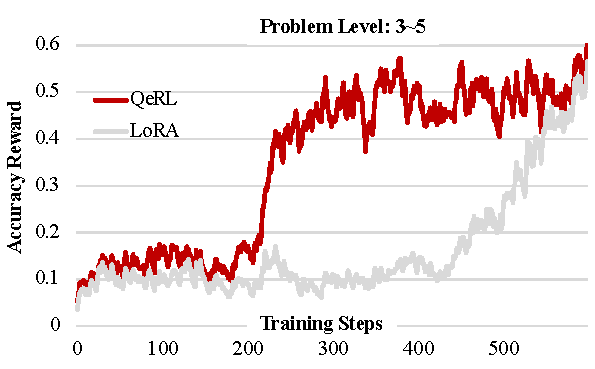
\includegraphics[width=\textwidth]{figures/appendix_7B.pdf}
        \vspace{-0.2in}
        \caption{Training reward of 7B model.}
        \label{fig:ap_7b}
    \end{minipage}
    % 右图
        \hspace{0.1in}
    \begin{minipage}{0.45\textwidth}
        \centering
        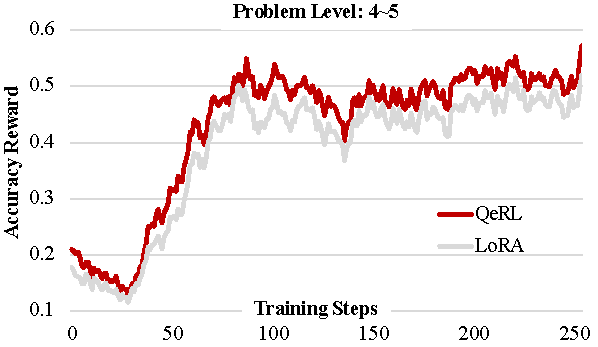
\includegraphics[width=\textwidth]{figures/appendix_32B.pdf}
        \vspace{-0.2in}
        \caption{Training reward of 32B model.}
        \label{fig:ap_32b}
    \end{minipage}
    } % 缩放结束
\vspace{-0.1in}
\end{figure}



\paragraph{Training Rewards of Different Model}\label{ap:more_reward}
Fig.\ref{fig:ap_7b} and Fig.\ref{fig:ap_32b} further compare the performance of QeRL and 16-bit LoRA training on complex reasoning datasets. In Fig.\ref{fig:ap_7b}, we present the training rewards of the Qwen2.5-7B-Instruct model on the BigMath dataset with difficulty levels ranging from 3 to 5, as an extension of Fig.\ref{fig:bigmath}. Leveraging the exploration benefits of QeRL in quantized models, a rapid increase in reward is observed after approximately 200 steps, whereas 16-bit LoRA requires over 500 steps to achieve a similar rise. Meanwhile, as shown in Fig.\ref{fig:ap_32b}, we trained the Qwen2.5-32B-Instruct model on the highest difficulty data (levels 4–5). Although the difference in reward growth between QeRL and LoRA is less pronounced in the 32B model compared to the smaller 3B, 7B, and 14B models, QeRL still consistently performs better than LoRA.

\paragraph{More Experiments of Entropy}\label{ap:more_entropy}

\begin{wrapfigure}{h}{0.4\textwidth}
\vspace{-0.2in}
    \centering
    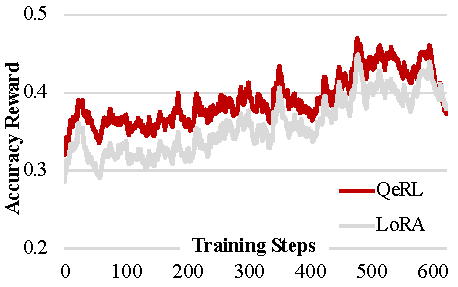
\includegraphics[width=0.4\textwidth]{figures/app_entropy.pdf} 
    \vspace{-0.2in}
    \caption{
        Entropy in RL steps. 
    }
    \label{fig:ap_entropy}
\vspace{-0.2in}
\end{wrapfigure}

As an extension of Fig.\ref{fig:entropy}, Fig.\ref{fig:ap_entropy} illustrates the entropy curve of the Qwen2.5-14B-Instruct model at various training steps. Notably, the entropy of QeRL remains consistently higher than that of LoRA throughout the RL process, particularly during the initial steps. This observation highlights the advantage of QeRL in promoting exploration during RL, as higher entropy indicates a broader search of the solution space. The increased exploratory capacity facilitated by quantization appears to enable the model to navigate complex environments more effectively, ultimately supporting improved optimization. These results further validate the role of quantization in enhancing the exploration-exploitation balance in RL tasks.


\paragraph{Noise Scheduler}\label{ap:noise}

\begin{wrapfigure}{h}{0.5\textwidth}
\vspace{-0.1in}
    \centering
    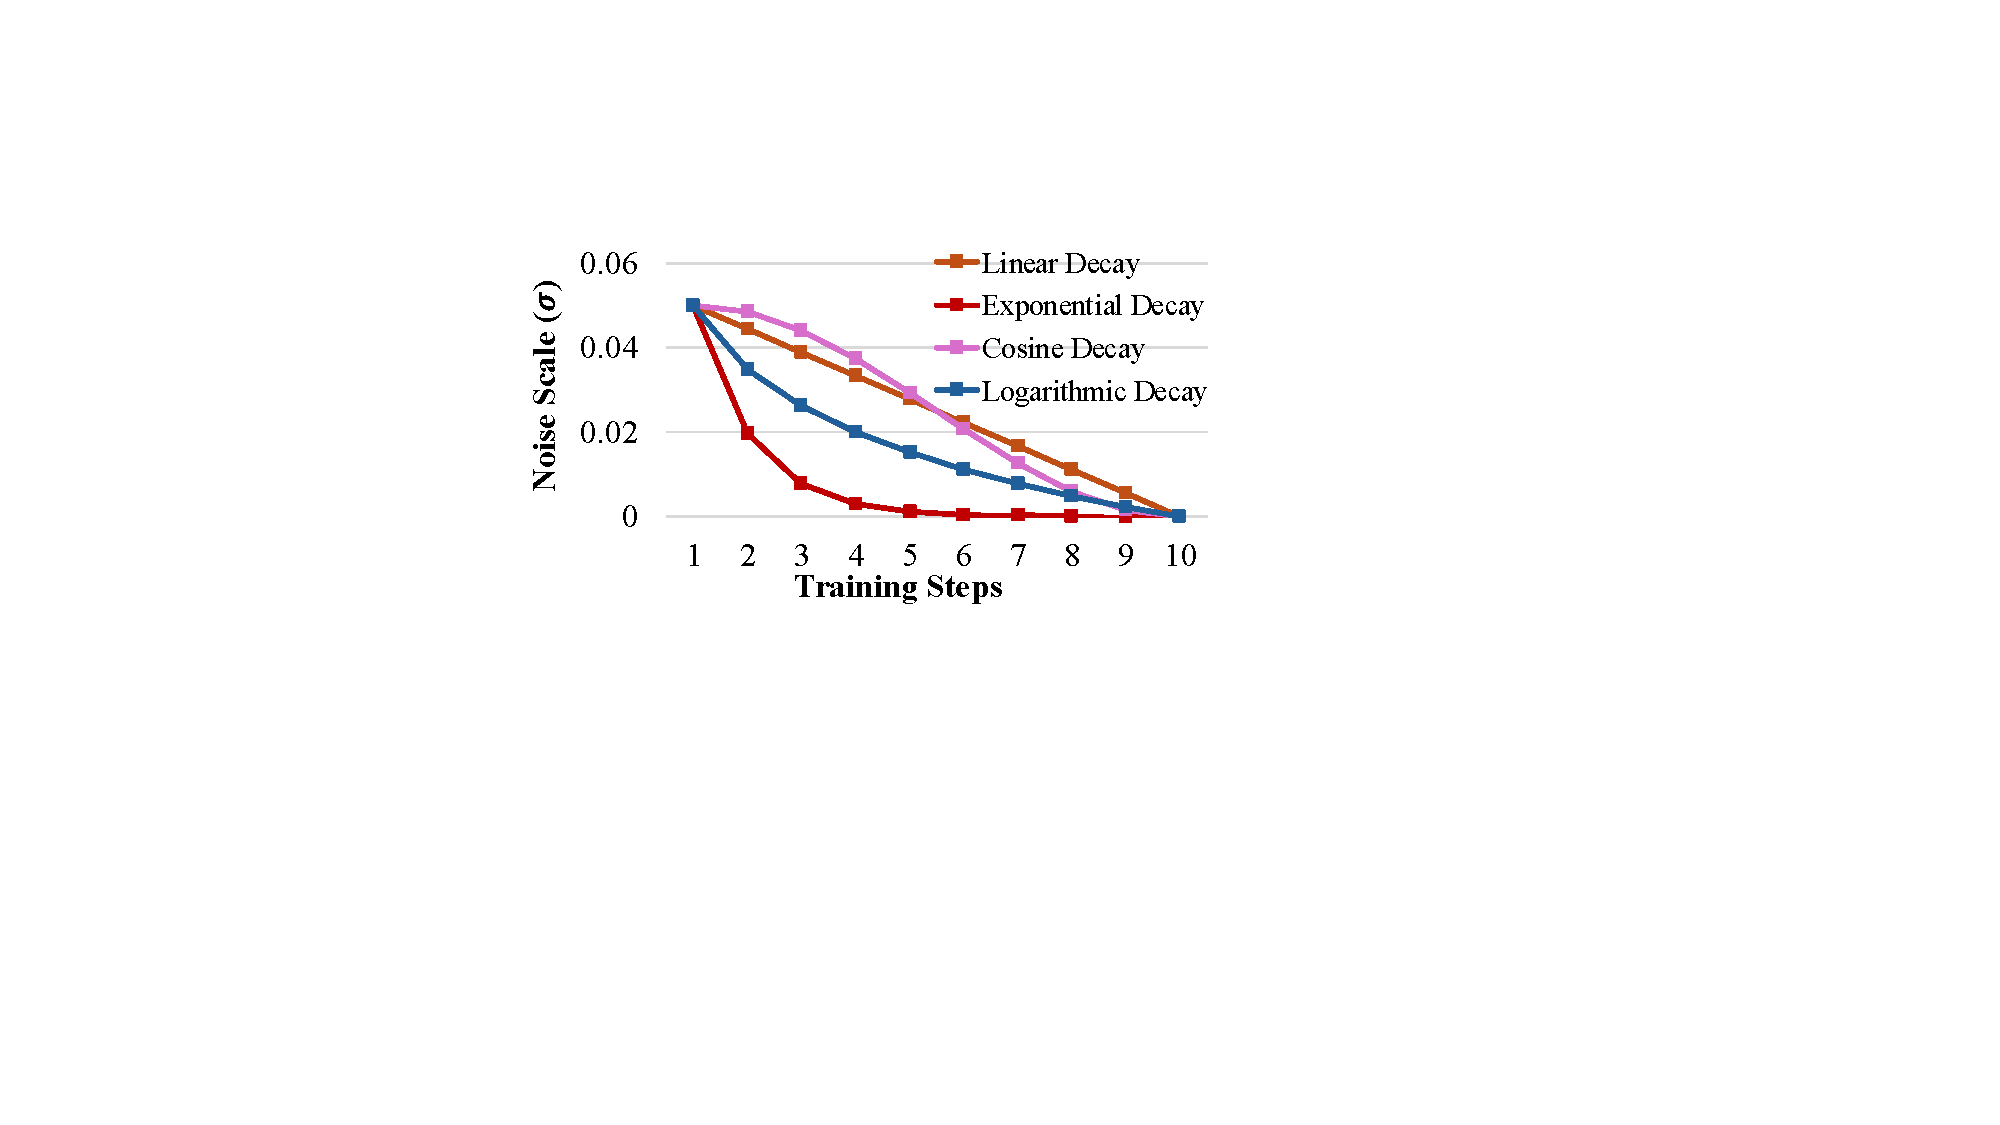
\includegraphics[width=0.5\textwidth]{figures/decay_curve_v2.pdf} 
    \vspace{-0.2in}
    \caption{
        Noise curve of different schedulers. 
    }
    \label{fig:decay_curve_ablation}
\vspace{-0.1in}
\end{wrapfigure}

Fig.\ref{fig:decay_curve_ablation} illustrates the noise scheduler employed in our experiments, showing four distinct decay strategies: linear, exponential, cosine, and logarithmic. The scheduler adjusts the noise level in 10 stages to guide the training process. The linear decay method reduces noise uniformly across stages, ensuring a consistent rate of change. The exponential decay rapidly decreases the noise at the beginning and uses smaller noise scales in later stages, which we found effective for achieving stable and higher rewards in later stages of training. The cosine decay follows a smooth oscillatory pattern, gradually reducing noise with a cosine curve, whereas the logarithmic decay decreases noise sharply in early stages and stabilizes in later ones. Among these, we chose the exponential decay strategy due to its ability to maintain smaller noise scales during the later stages, resulting in a more stable and higher reward curve. This flexibility in controlling noise levels plays a critical role in balancing exploration and convergence during training.

\section{Additional Ablation Study}\label{ap:rank}

\begin{figure}[t]
\vspace{-0.1in}
    \centering
    \scalebox{1}{ % 缩放开始
    % 左图
    \begin{minipage}{0.45\textwidth}
        \centering
        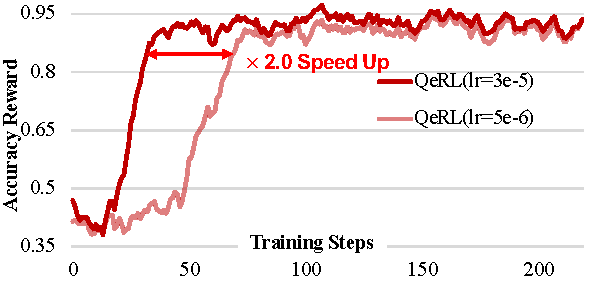
\includegraphics[width=\textwidth]{figures/appendix_lr_qerl.pdf}
        \vspace{-0.2in}
        \caption{Ablation of learning rate in QeRL (Qwen2.5-7B-Instruct).}
        \label{fig:ap_lr_qerl}
    \end{minipage}
    % 右图
        \hspace{0.1in}
    \begin{minipage}{0.45\textwidth}
        \centering
        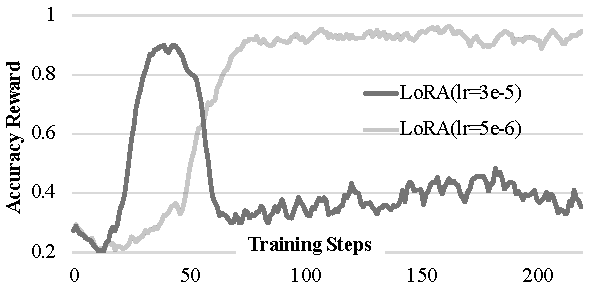
\includegraphics[width=\textwidth]{figures/appendix_lr_lora.pdf}
        \vspace{-0.2in}
        \caption{Ablation of learning rate in LoRA (Qwen2.5-7B-Instruct).}
        \label{fig:ap_lr_lora}
    \end{minipage}
    } % 缩放结束
\vspace{-0.1in}
\end{figure}

\textbf{Ablation of Learning Rate} We examine the impact of learning rate variations on the performance of quantized models compared to 16-bit models. As illustrated in Fig.\ref{fig:ap_lr_qerl} and Fig.\ref{fig:ap_lr_lora}, with a relatively small learning rate of 5e-6, QeRL marginally outperforms LoRA, achieving a reward close to 0.95. When the learning rate is increased to 3e-5, the larger update magnitude in the adapter results in faster reward growth and quicker model convergence. However, in 16-bit models, the excessive update magnitude leads to instability, often causing the training process to collapse. In contrast, QeRL demonstrates remarkable robustness to larger learning rates due to the presence of NVFP4 quantization noise, which helps stabilize updates. This robustness enables QeRL to maintain stable training even under high learning rates, achieving a reward growth rate nearly twice as fast as the 16-bit model. These results underscore QeRL's superior adaptability and efficiency, particularly in challenging training scenarios with high learning rates.

\section{More Efficiency Experiments}\label{ap:efficient}

\begin{table}[t]
\centering
\begin{tabular}{cccccccc}
\toprule
\multirow{2}{*}{\textbf{Method}} & \multirow{2}{*}{\textbf{W\#}} & \multirow{2}{*}{\textbf{Model Size}} & \multirow{2}{*}{\textbf{BS\#}} & \multicolumn{2}{c}{\textbf{Throughput (Tokens/s)}} & \multicolumn{2}{c}{\textbf{E2E RL Speedup}} \\
\cmidrule(lr){5-6}\cmidrule(lr){7-8}
&&&& Rollout Phase & Speedup & w/o GC & w/ GC \\
\midrule
LoRA & BF16  & 6.2 GB & 2 & 151.2 & - & - & - \\
\textbf{QeRL} & \textbf{NVFP4} & 2.8 GB & 2 & \textbf{157.0} & $\textcolor{hanred}{\times\mathbf{1.0}}$ & $\textcolor{hanred}{\times\mathbf{1.1}}$ & $\textcolor{hanred}{\times\mathbf{1.0}}$ \\
\midrule \midrule
LoRA & BF16  & 6.2 GB & 8 & 2226.3 & - & - & - \\
\textbf{QeRL} & \textbf{NVFP4} & 2.8 GB & 8 & \textbf{2271.4} & $\textcolor{hanred}{\times\mathbf{1.0}}$ & $\textcolor{hanred}{\times\mathbf{1.1}}$ & $\textcolor{hanred}{\times\mathbf{1.1}}$ \\
\bottomrule
\end{tabular}
\caption{Memory Saving and Speedup of Qwen2.5-3B-Instruct Model. The table reports the throughput (tokens/s) for the rollout phase under two batch size settings (2 and 8). Each input has a length of 256 tokens, and each max completion length is 2048. ``W\#'' denotes the data format, ``BS\#'' is the number of batch size, and ``E2E'' denotes the end-to-end speed of GRPO training. ``GC'' denotes gradient checkpointing.}
\label{tab:efficiency_3b}
\end{table}


\begin{table}[!t]
\centering
%\resizebox{\columnwidth}{!}{
\begin{tabular}{cccccccc}
\toprule
\multirow{2}{*}{\textbf{Method}} & \multirow{2}{*}{\textbf{W\#}} & \multirow{2}{*}{\textbf{Model Size}} & \multirow{2}{*}{\textbf{BS\#}} & \multicolumn{2}{c}{\textbf{Throughput (Tokens/s)}} & \multicolumn{2}{c}{\textbf{E2E RL Speedup}} \\ 
\cmidrule(lr){5-6}\cmidrule(lr){7-8}
&&&& Rollout Phase & Speedup & w/o GC & w/ GC \\
\midrule
% \multirow{6}{*}{\makecell{7B}} 
LoRA&BF16  & 15.2 GB& 2 & 115.4 & - & - & - \\  
%\cdashline{1-7}
\textbf{QeRL}&\textbf{NVFP4}  & 5.9 GB& 2  & \textbf{151.6}&$\textcolor{hanred}{\times\mathbf{1.3}\uparrow}$&$\textcolor{hanred}{\times\mathbf{1.2}\uparrow}$&$\textcolor{hanred}{\times\mathbf{1.2}\uparrow}$  \\ 
\midrule \midrule
LoRA&BF16  &15.2 GB& 8 &1641.1& - & - & - \\ 
%\cdashline{1-7}
\textbf{QeRL}&\textbf{NVFP4}  & 5.9 GB& 8 & \textbf{2091.8}&$\textcolor{hanred}{\times\mathbf{1.3}\uparrow}$&$\textcolor{hanred}{\times\mathbf{1.1}\uparrow}$&$\textcolor{hanred}{\times\mathbf{1.1}\uparrow}$ \\ 
\bottomrule
\end{tabular}
%}
\caption{Memory Saving and Speedup of Qwen2.5-7B-Instruct Model. The table reports the throughput (tokens/s) for the rollout phase under two batch size settings (2 and 8). Each input has a length of 256 tokens, and each max completion length is 2048. ``W\#'' denotes the data format, ``BS\#'' is the number of batch size, and ``E2E'' denotes the end-to-end speed of GRPO training. ``GC'' denotes gradient checkpointing.} \label{tab:efficiency_7b}
\end{table}




\begin{table}[!t]
\centering
%\resizebox{\columnwidth}{!}{
\begin{tabular}{cccccccc}
\toprule
\multirow{2}{*}{\textbf{Method}} & \multirow{2}{*}{\textbf{W\#}} & \multirow{2}{*}{\textbf{Model Size}} & \multirow{2}{*}{\textbf{BS\#}} & \multicolumn{2}{c}{\textbf{Throughput (Tokens/s)}}&\multicolumn{2}{c}{\textbf{E2E RL Speedup}} \\ 
\cmidrule(lr){5-6}\cmidrule(lr){7-8}
&&&& Rollout Phase & Speedup & w/o GC & w/ GC \\
\midrule
% \multirow{6}{*}{\makecell{7B}} 
LoRA&BF16  & 29.6 GB& 2 & 65.4 & - & - & - \\  

%\cdashline{1-7}
\textbf{QeRL}&\textbf{NVFP4}  & 10.6 GB& 2  & \textbf{95.3}&$\textcolor{hanred}{\times\mathbf{1.3}\uparrow}$&$\textcolor{hanred}{\times\mathbf{1.4}\uparrow}$ &$\textcolor{hanred}{\times\mathbf{1.4}\uparrow}$ \\ 
\midrule \midrule
LoRA&BF16  &29.6 GB& 8 &737.2& - & OOM & - \\ 

%\cdashline{1-7}
\textbf{QeRL}&\textbf{NVFP4}  &10.6 GB& 8 &\textbf{1091.1}&$\textcolor{hanred}{\times\mathbf{1.5}\uparrow}$& OOM &$\textcolor{hanred}{\times\mathbf{1.3}\uparrow}$ \\ 
\bottomrule
\end{tabular}
%}
\caption{Memory Saving and Speedup of Qwen2.5-14B-Instruct Model. The table reports the throughput (tokens/s) for the rollout phase under two batch size settings (2 and 8). Each input has a length of 256 tokens, and each max completion length is 2048. ``W\#'' denotes the data format, ``BS\#'' is the number of batch size, and ``E2E'' denotes the end-to-end speed of GRPO training. ``GC'' denotes gradient checkpointing.} \label{tab:efficiency_14b}
% \vspace{-0.1in}
\end{table}

\begin{table}[!t]
\centering
\begin{tabular}{cccccccc}
\toprule
\multirow{2}{*}{\textbf{Method}} & \multirow{2}{*}{\textbf{W\#}} & \multirow{2}{*}{\textbf{Model Size}} & \multirow{2}{*}{\textbf{BS\#}} & \multicolumn{2}{c}{\textbf{Throughput (Tokens/s)}}&\multicolumn{2}{c}{\textbf{E2E RL Speedup}} \\ 
\cmidrule(lr){5-6}\cmidrule(lr){7-8}
&&&& Rollout Phase & Speedup & w/o GC & w/ GC \\
\midrule
% \multirow{6}{*}{\makecell{14B}} 
LoRA&BF16  & 62.3 GB& 2 & 34.0 & - & OOM & OOM \\  
%\cdashline{1-7}
\textbf{QeRL}&\textbf{NVFP4}  & 20.7 GB& 2  & \textbf{60.0}&$\textcolor{hanred}{\times\mathbf{1.8}}$& OOM & 10.6 s/step \\ 
\midrule \midrule
LoRA&BF16  &62.3 GB& 8 &344.3& - & OOM & OOM\\ 
\textbf{QeRL}&\textbf{NVFP4}   &  20.7 GB& 8 &\textbf{688.2}&$\textcolor{hanred}{\times\mathbf{2.0}}$& OOM & 12.2 s/step\\ 
\bottomrule
\end{tabular}
\caption{Memory Saving and Speedup of Qwen2.5-32B-Instruct Model. The table reports the throughput (tokens/s) for the rollout phase under two batch size settings (2 and 8). Each input has a length of 256 tokens, and each max completion length is 2048. ``W\#'' denotes the data format, ``BS\#'' is the number of batch size, and ``E2E'' denotes the end-to-end speed of GRPO training. ``GC'' denotes gradient checkpointing.} \label{tab:efficiency_32b}
\end{table}

\begin{table}[!t]
\centering
% First table (Qwen2.5-3B)
\begin{minipage}{0.45\textwidth} 
\begin{tabular}{rrrr}
\toprule
\textbf{Model} & \multicolumn{3}{c}{\textbf{BF16 (Tokens/s)}}\\ 
\cmidrule(lr){2-4}
               & Rank 16 & Rank 32 & Rank 64\\ 
\midrule
3B    & 151.2  & 148.8  & 138.6\\ 
7B    & 115.4 & 113.2 & 108.3\\ 
14B   & 65.4 & 63.1 & 61.2 \\ 
32B   & 34.0 & 33.3 & 31.9 \\ 
\bottomrule
\end{tabular}
\label{tab:example_table}
\end{minipage}% <-- 注意这里没有空行
\hfill % 在表格之间添加水平弹性空间
% Second table (Qwen2.5-7B)
\begin{minipage}{0.45\textwidth}
\begin{tabular}{rrrr}
\toprule
\textbf{Model}& \multicolumn{3}{c}{\textbf{NVFP4 (Tokens/s)}}\\ 
\cmidrule(lr){2-4}
    & Rank 16 & Rank 32 & Rank 64\\ 
\midrule
3B     & 157.0  & 153.1  & 140.0\\ 
7B     & 151.6 & 149.9 & 137.7\\ 
14B    & 95.3 & 92.9 & 86.0 \\ 
32B    & 58.0 & 56.0 & 51.3 \\ 
\bottomrule
\end{tabular}
\end{minipage}% <-- 注意这里没有空行
\caption{Throughput under different LoRA ranks in the rollout stage. We test the tokens/s for each model in the vLLM engine, and the setting is aligned with Tab.\ref{tab:efficiency_14b}. We set the batch size as 1.}
\label{tab:throughput_rank}
\end{table}


Tab.\ref{tab:efficiency_3b}, Tab.\ref{tab:efficiency_7b}, Tab.\ref{tab:efficiency_14b}, and Tab.\ref{tab:efficiency_32b} provide additional speed benchmarks for the Qwen2.5-3B-Instruct, Qwen2.5-7B-Instruct, Qwen2.5-14B-Instruct, and Qwen2.5-32B-Instruct models, evaluated under batch sizes of 2 and 8. For the 3B and 7B models, we did not enable memory-efficient techniques such as gradient checkpointing~\citep{chen2016training} or Liger loss~\citep{hsu2025ligerkernel} in order to maximize training speed. However, due to the substantial size of the 14B and 32B models and the computational overhead introduced by importance sampling with gradients during RL training, we employ gradient checkpoint to accelerate computation. For training on GPUs with smaller memory capacity, enabling gradient checkpointing is recommended to reduce memory usage, although this may come at the cost of slower overall training speed. During the rollout phase, the precision of NVFP4, optimized by the Marlin kernel~\citep{frantar2024marlin}, demonstrates a significant acceleration, achieving speeds of 1.0 to 2.0$\times$. In particular, performance gains become more pronounced as model size increases, with the 32B model achieving up to a 2.0$\times$ speedup. This indicates that NVFP4's advantages are particularly impactful for large-scale models, where computational demands are higher.

In end-to-end RL efficiency evaluation, we report the per-step latency of GRPO training, defined as the wall clock time to complete an optimization step including rollout generation, log-probability computation, and parameter updates. We benchmark with rollout batch sizes of 2 and 8 while fixing the maximum input length to 256 tokens and the maximum completion length to 2,048 tokens. For fairness, we match the vLLM memory budget between BF16 and NVFP4 variants by setting the same gpu memory utilization in the engine: 0.20 for Qwen2.5-3B-Instruct, 0.30 for 7B, 0.45 for 14B, and 0.40 for 32B (the latter to enable single-GPU training). Under these controlled settings, the E2E latency reductions mirror the rollout phase acceleration and become more pronounced as the model size grows, with the largest gains observed on Qwen2.5-14B-Instruct.

Additionally, Tab.\ref{tab:throughput_rank} provides a comparison of inference speeds between 16-bit and NVFP4 main models across various LoRA ranks. NVFP4 consistently outperforms 16-bit models in terms of speed at all adapter ranks, showcasing its ability to maintain efficiency across diverse configurations. However, as the rank increases, both NVFP4 and BF16 experience a gradual decline in rollout speed within the vLLM engine, likely due to the increased computational overhead associated with higher ranks. Despite this, NVFP4 continues to demonstrate superior performance, highlighting its robustness and adaptability for both small-scale and large-scale setups. These findings underscore NVFP4's potential to optimize inference efficiency, particularly when combined with advanced kernels and varying adapter configurations.

\section{Limitation Analysis}

We have demonstrated that our method, QeRL, achieves superior performance in RL training for LLMs compared to 16-bit vanilla LoRA training. Additionally, QeRL matches the accuracy of 16-bit full-parameter reinforcement fine-tuning while delivering over 2$\times$ training speedup relative to both vanilla LoRA and QLoRA. However, since RL for LLMs inherently demands significantly greater computational resources than SFT, our experiments, conducted on model sizes ranging from 3B to 32B, do not yet establish whether QeRL can maintain the same level of performance for models exceeding 70B parameters, leaving that investigation for future work. Another limitation is that RL training often requires tens or even hundreds of hours, and while we have provided comprehensive evaluations on reasoning benchmarks such as GSM8K, MATH 500, AIME 24, AIME 25, and AMC 23, we did not extend our evaluations to other benchmarks or data types, such as code, or to general-purpose language tasks unrelated to reasoning. Nevertheless, our technique can be seamlessly adapted to richer and more diverse training datasets. We encourage the community to explore and apply this method to a broader range of tasks in future research.


